\documentclass[10pt,twocolumn,letterpaper]{article}
\usepackage[pagenumbers]{cvpr}
\usepackage[T1]{fontenc}
\usepackage{times,graphicx,amsmath,amssymb,booktabs,multirow}
\usepackage[breaklinks,colorlinks,citecolor=blue,urlcolor=blue]{hyperref}
\def\confName{CVPR}\def\confYear{2027}
\title{Position-Conditioned Deformation Prediction with Unknown Material and Environmental Interactions}
\author{Anonymous authors\\Research manuscript draft}
\begin{document}
\raggedbottom
\maketitle
\begin{abstract}
Predicting deformation from visual observations requires distinguishing an object's material response from the effects of its environment. Similar observed motions can result from different combinations of elasticity, fixture compliance, gravity, and spatial loading. We study position-conditioned prediction: a model observes a short sequence of object positions and prescribed tool poses, then predicts deformation under a new positional interaction without receiving the true force history. Our formulation separates object-attached material properties from environmental interaction fields and fits their latent parameters through implicitly differentiated nonlinear equilibrium. We develop a controlled benchmark that separates familiar positional motions from held-out interaction families and evaluates prediction before and after additional observations. Numerical reference checks and matched observation interfaces support comparisons with physical digital-twin methods and learned positional predictors. Quantitative conclusions in the final manuscript will be generated from the completed, frozen evaluation.
\end{abstract}

\begin{figure*}[t]
\centering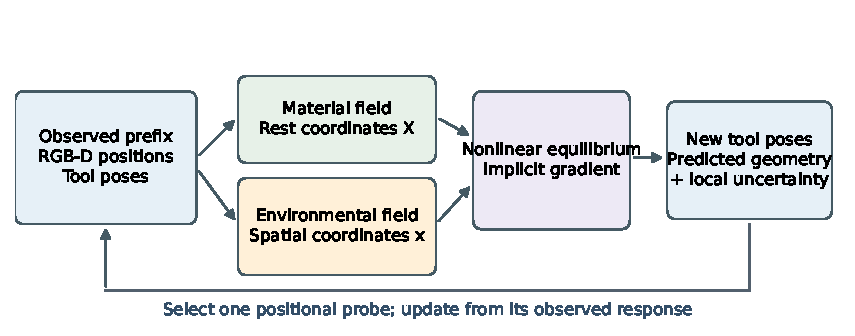
\includegraphics[width=\textwidth]{figures/method.pdf}
\caption{Position-conditioned inverse mechanics. Observed object positions constrain material and environmental explanations. New tool poses are converted to interaction through the inferred model; true force histories are not supplied. Local predictive sensitivities support selecting an additional observation.}
\label{fig:method}
\end{figure*}

\section{Introduction}
Physical digital twins connect visual reconstruction to predictions about how an object responds to interaction. A useful twin should answer a positional query: if a gripper moves here, or a tool follows this trajectory, how will the object deform? The reaction forces are consequences of the interaction, rather than necessarily available inputs. This distinction matters when deploying a model without calibrated force sensing.

Material properties alone do not determine the observed response. Fixtures may deform, constraints may be only partially visible, and distributed forces may act throughout the volume. A model that explains an observed trajectory by changing material stiffness can reproduce that trajectory while predicting a different interaction incorrectly. The resulting ambiguity is especially consequential outside the interaction patterns used for reconstruction.

We investigate a spatially factored model of this problem. Material coordinates index the object, while environmental interactions are evaluated at the current spatial positions and tool poses. This representation makes the action interface positional and allows forces to emerge from the inferred interaction model. We evaluate generalization across explicitly declared interaction groups rather than treating additional noisy observations of the same motion as independent out-of-distribution evidence.

We contribute a spatially factored positional prediction protocol, an independently refined simulation benchmark with separate material and environmental shifts, and matched-information tests of prediction and one-observation adaptation.

Our study builds on complementary advances in physical Gaussian representations and visual system identification. PhysGaussian~\cite{xie2024physgaussian} couples continuum simulation and Gaussian rendering, while PhysTwin~\cite{jiang2025phystwin} reconstructs visual and physical object models from interaction videos. These systems establish strong tools for building and using digital twins. Our experiments target the additional question of how unknown environmental interactions affect positional generalization, and how limited new observations can resolve those ambiguities.

\section{Related Work}
\paragraph{Physical visual representations.}
PhysGaussian~\cite{xie2024physgaussian} integrates 3D Gaussian rendering with material-point simulation. Its representation supports a broad range of material behaviors and prescribed scene interactions. PhysTwin~\cite{jiang2025phystwin} combines spring-mass simulation, geometric reconstruction, and Gaussian appearance modeling to infer deformable twins from sparse interaction videos. We compare compatible physical prediction components under a common observation interface and identify adaptations explicitly; our controlled experiments do not substitute for an evaluation of every capability of these complete systems.

\paragraph{Learning physical response.}
Spring-Gaus~\cite{zhong2024springgaus} identifies elastic spring-mass models from video and evaluates future simulation under changed initial states and environmental parameters. PhysDreamer~\cite{zhang2024physdreamer} uses video-generation priors to estimate spatial material fields and synthesize plausible interactions. UniPhy~\cite{mittal2025uniphy} learns a shared latent-conditioned constitutive model across elastic, plastic, granular, and fluid materials, then optimizes a latent from observed positions for re-simulation under new conditions. These results establish that material inference and interaction generalization are already important capabilities of existing work. Our controlled study addresses their interaction with unknown environmental explanations and the selection of additional positional observations. Our focus is the ambiguity between material response and spatial interaction, and its consequences for positional queries.

\paragraph{Acquiring informative interactions.}
AuRA~\cite{yu2026aura} automates robot interaction and data preparation for deformable digital-twin reconstruction. Its focus on efficient acquisition complements our study of uncertainty in the physical explanation of an observed interaction. We distinguish initial generalization from adaptation after collecting additional observations, and report acquisition and computational costs separately.

\section{Problem Formulation}
Let $X\in\Omega_0$ denote a material point in a canonical object, and let $x(X,a)=X+u(X,a)$ be its spatial position under a positional action $a$. The action specifies tool translations and rotations. An observed prefix $\mathcal D=\{a_j,y_j\}_{j=1}^m$ contains partial position observations obtained through the visual pipeline. The prediction task is to estimate $u(X,a_*)$ for an unseen action $a_*$, together with predictive uncertainty when supported by the fitted model.

The latent variables are divided into material parameters $\theta_m$ and environmental parameters $\theta_e$. True reaction forces and simulator material labels are excluded from the primary model inputs. Privileged experiments that supply such labels are reported separately. Known geometry and camera calibration are explicit assumptions of the controlled protocol.

\section{Spatially Factored Inverse Mechanics}
\subsection{Position-driven equilibrium}
We model settled deformation as a stationary point of total potential energy,
\begin{align}
 u^*(a,\theta)&=\arg\min_u\Pi(u,a,\theta),\\
 \Pi&=\int_{\Omega_0}W(F;\theta_m)\,dX
\nonumber\\
 &\quad+\sum_k\frac12\int_{\Gamma_k}\kappa_k(X)\|u-d_k(a)\|^2\,dS\nonumber\\
 &\quad-\int_{\Omega_0}\rho g^\top u\,dX
 +\int_{\Omega_0}\phi(X+u;\theta_e)\,dX.\label{eq:energy}
\end{align}
Here $F=I+\nabla_Xu$, $d_k(a)$ is the displacement prescribed by a rigid tool pose, and $\kappa_k$ represents compliant coupling to that tool or fixture. Gravity is a body force; surface constraints and spatial loading retain their distinct physical roles. The potential $\phi$ is evaluated in spatial coordinates, so its force changes as material moves through the environment.

The initial constitutive implementation uses a compressible Neo-Hookean energy,
\begin{multline}
 W(F)=\frac\mu2(\mathrm{tr}(F^\top F)-3)-\mu\log J
       \\
 +\frac\lambda2(\log J)^2,\qquad J=\det F.
\end{multline}
The simulator enforces a positive-Jacobian guard and checks equilibrium residuals. Reference solutions use quadratic finite elements with spatial and quadrature refinement. Displacement qualification does not imply convergence of every derived stress or traction quantity.

\subsection{Material and environmental fields}
The material field is attached to the reference object. In the controlled study,
\begin{equation}
 E(X)=E_0\exp\!\left[h\left(b_1(X)-b_2(X)\right)\right],
\end{equation}
where $b_i$ are fixed radial basis functions along the block's length. The coefficient $h$ controls spatial stiffness variation. The environmental potential is a spatial Gaussian, $\phi(x)=A|\Omega_0|^{-1}\exp(-\|x-c\|^2/(2s^2))$, with inferred energy amplitude $A$, center $c$, and width $s$. Its force is $-\nabla_x\phi(x)$ and changes as the object traverses the field. Two compliant surface footprints couple the object to the position-controlled tools. Each footprint is a Gaussian in the end-face coordinates, tapered to zero at the perimeter. We infer its total stiffness $K_k$ and select among three footprint-layout hypotheses. With nonnegative footprint $w_k(X)$,
\begin{equation}
 \kappa_k(X)=\frac{K_kw_k(X)}{\int_{\Gamma_k}w_k(X)\,dS}.
\end{equation}
The normalization separates contact location from total coupling stiffness. The smooth finite footprint also avoids an abrupt traction transition at an idealized half-face attachment.

Gravity has known magnitude and unknown direction in the observation frame. Density, Poisson ratio, canonical geometry, and tool kinematics are shared known quantities. Thus the study isolates uncertainty in stiffness, attachment, and environmental loading. Material OOD tests change elastic coefficients and heterogeneity within this constitutive family.

\subsection{Inference from positional observations}
For an observation operator $H_j$, we fit latent parameters by minimizing a position discrepancy,
\begin{equation}
 \mathcal L(\theta)=\sum_j\|H_j \hat u(a_j,\theta)-y_j\|^2_{\Sigma_j^{-1}}+\|z-z_0\|^2_{\Lambda}.
\end{equation}
Here $z$ denotes scaled latent coordinates, with log coordinates for positive stiffnesses and field width. Weak regularization constrains poorly identified directions. We screen the three attachment layouts using a coarse model and refine layouts within one normalized loss unit of the best candidate. Parameter bounds and initialization are selected on development cases before the held-out evaluation. The predictor receives the positional action, not the forces computed internally by the equilibrium model.

Let $R(u,\theta,a)=\partial\Pi/\partial u$ and $K=\partial R/\partial u$. At a nonsingular equilibrium, an adjoint solve gives
\begin{equation}
 K^\top v=\frac{\partial\mathcal L}{\partial u},\qquad
 \frac{d\mathcal L}{d\theta}=-v^\top\frac{\partial R}{\partial\theta}.
\end{equation}
We verify the implementation against an independent sparse assembly and finite differences of the equilibrium solution.

\paragraph{Reducing forward discretization bias.}
A coarse forward model can explain its own numerical error by changing material or environmental parameters. We therefore combine equilibrium predictions at two resolutions,
\begin{equation}
 \hat u=\frac{9u_3-4P_{2\to3}u_2}{5},
\end{equation}
where $u_n$ uses $4n\times n\times n$ quadratic elements and $P_{2\to3}$ interpolates the coarse field. This removes a leading quadratic resolution term when that error model applies. We assess the correction on development oracle cases, differentiate both equilibrium solves, and retain a positive-Jacobian check on the corrected field. The corrected field approximates the continuum response; remaining discrepancy is included in predictive calibration.

\subsection{Predictive sensitivity and probing}
Let $J_a=\partial \hat u(a,\hat\theta)/\partial z$ denote the positional sensitivity at the fitted explanation. We construct a regularized local covariance
\begin{equation}
 C=\left(J_{\mathcal D}^{\top}\Sigma^{-1}J_{\mathcal D}+\Lambda\right)^{-1},
\end{equation}
where $\Lambda$ encodes weak parameter-scale regularization. This local approximation describes sensitivity around a fitted explanation. A separate object-level calibration stage sets the predictive interval scale.

For a candidate probe $a$, observing its visible points yields an approximate covariance $C_a=(C^{-1}+J_a^{\top}H_a^{\top}\Sigma^{-1}H_aJ_a)^{-1}$. We choose the probe that maximizes the reduction in target predictive variance,
\begin{equation}
 a^*=\arg\max_a\mathrm{tr}\!\left[J_*\left(C-C_a\right)J_*^{\top}\right].
\end{equation}
Probe selection uses predicted sensitivities, without observing candidate responses. The selected response is then acquired and the inverse problem is refitted. A separate target interaction remains unobserved throughout adaptation.

\paragraph{Object-level calibration.}
For each calibration object, we take the 90th percentile of absolute held-action coordinate errors divided by $\sqrt{\sigma^2+\epsilon^2}$, where $\sigma^2=\operatorname{diag}(J_aCJ_a^\top)$ and $\epsilon=20\,\mu$m is a fixed scale floor. The order statistic at rank $\lceil0.9(n+1)\rceil$ of the $n$ object scores determines a common interval multiplier. Under object exchangeability, this construction targets at least 90\% coordinate coverage for 90\% of objects. We measure both coordinate and object coverage on each OOD cohort; exchangeability with the calibration distribution is not assumed for these shifts.

\subsection{Generalization and adaptation}
We distinguish three questions: prediction under a new action before its response is observed; calibration of uncertainty about that response; and prediction after a limited adaptation budget. A completely unobserved change in external loading is not assumed to be uniquely predictable from position alone. Such changes are evaluated through detection and adaptation, with the information available to each method stated explicitly.

\section{Experimental Protocol}
\paragraph{Draft status.} Experiments are in progress. Counts below describe the registered protocol, not completed evaluations. Final tables will distinguish completed results, numerical qualification, and any failures.

\paragraph{Geometry and observations.}
The controlled object is a $240\times80\times80$\,mm deformable block with known canonical geometry, density $625$\,kg/m$^3$, and Poisson ratio $0.35$. Two position-controlled tools couple to unknown smooth Gaussian attachment footprints. The observed prefix contains three settled configurations: nominal tool poses, a 6\,mm right-tool translation along $y$, and a 6\,mm translation along $z$. A $640\times480$ rendered RGB-D marker pipeline provides the same 27 visible point positions to all methods. Known synthetic marker IDs establish correspondence; depth has independent 0.3\,mm Gaussian noise and image sampling introduces pixel quantization. The positional objective uses a common 0.3\,mm coordinate scale. No force, reaction, material, or attachment labels are supplied. Predictions are evaluated at 81 canonical query points, with visible and hidden-surface subsets reported separately.

\paragraph{Cohorts and shifts.}
The protocol declares nine development objects, twelve calibration objects, and three disjoint test cohorts: eighteen objects from the development parameter ranges, twelve with extrapolated elastic coefficients and spatial heterogeneity, and twelve with shifted environmental-field amplitude, center, width, and gravity direction. Material coefficients within development range from 8 to 40\,kPa, and total attachment stiffnesses from 1500 to 15000\,N/m. Each object has a new 3\,mm familiar-direction query, five new positional interaction patterns, and a doubled-amplitude query. New patterns include stretching, opposed tool motion, twisting, bending, and diagonal translation. An additional transfer challenge translates both tools together through the fixed spatial field. These are declared interaction and parameter shifts; the reference material law remains Neo-Hookean.

\paragraph{Numerical references.}
Reference geometry uses quadratic finite elements and independent spatial and quadrature refinement. Every action must have a displacement RMS change below 20\,$\mu$m, equilibrium residual below $10^{-9}$\,N, positive deformation Jacobians above $0.1$, and reaction balance below $10^{-7}$\,N. Maximum-coordinate refinement changes are retained separately, since localized attachment-edge behavior converges more slowly. Acceptance in an RMS norm does not certify pointwise stress convergence. The inverse predictor uses a smaller discretization and an independently checked dense tangent implementation. A development-only sharp-attachment pilot motivated the finite smooth footprint: its localized compression reached the Jacobian guard under refinement, whereas the smooth version retained substantial nonrigid deformation and passed the original numerical thresholds.

\paragraph{Comparisons.}
The physical baselines use official PhysTwin spring-mass and PhysGaussian material-point simulation components with documented adapters for the shared positional interface. They retain their own constitutive representations. PhysTwin learns per-spring parameters; the MPM adapter fits material variation, compliant tool coupling, and gravity direction. We tune initialization, discretization, and settling on development cases. A positional neural predictor is trained on a separate synthetic object bank, with an ID-action training variant and a separately reported variant exposed to all local action families. Controlled ablations fix environmental loading to its nominal value or freeze the spatial force at each material point's canonical position. The main predictor and neural comparisons cover all 42 declared test objects. The more expensive physical comparisons use the first six objects in each test cohort, giving two objects per attachment layout and an 18-object matched subset selected before test inference. Full Gaussian appearance reconstruction is outside this component benchmark.

\paragraph{Metrics and adaptation.}
The primary error is coordinate RMS displacement error,
\begin{equation}
 e=\sqrt{\frac{1}{3N}\sum_{i=1}^N\|\hat u_i-u_i\|_2^2}.
\end{equation}
We also report Euclidean point RMSE, hidden-surface error, and residual motion after removing the best rigid transform. Incremental error compares $\hat u(a)-\hat u(a_0)$ against $u(a)-u(a_0)$, separating the predicted response to the new action from static shape-completion error. Aggregation treats the object as the independent unit. Paired comparisons resample objects rather than frames or points. Probing compares a fixed $+40$\,mm $y$ translation, a reproducible random action, and the sensitivity-based policy, all with one additional acquired response and a separate $-40$\,mm $y$ target. Twelve independent calibration objects set separate pre- and post-acquisition interval scales; nine test objects evaluate transfer. A material-indexed-load ablation receives exactly the probe response selected for the spatial model.

\begin{figure*}[t]
\centering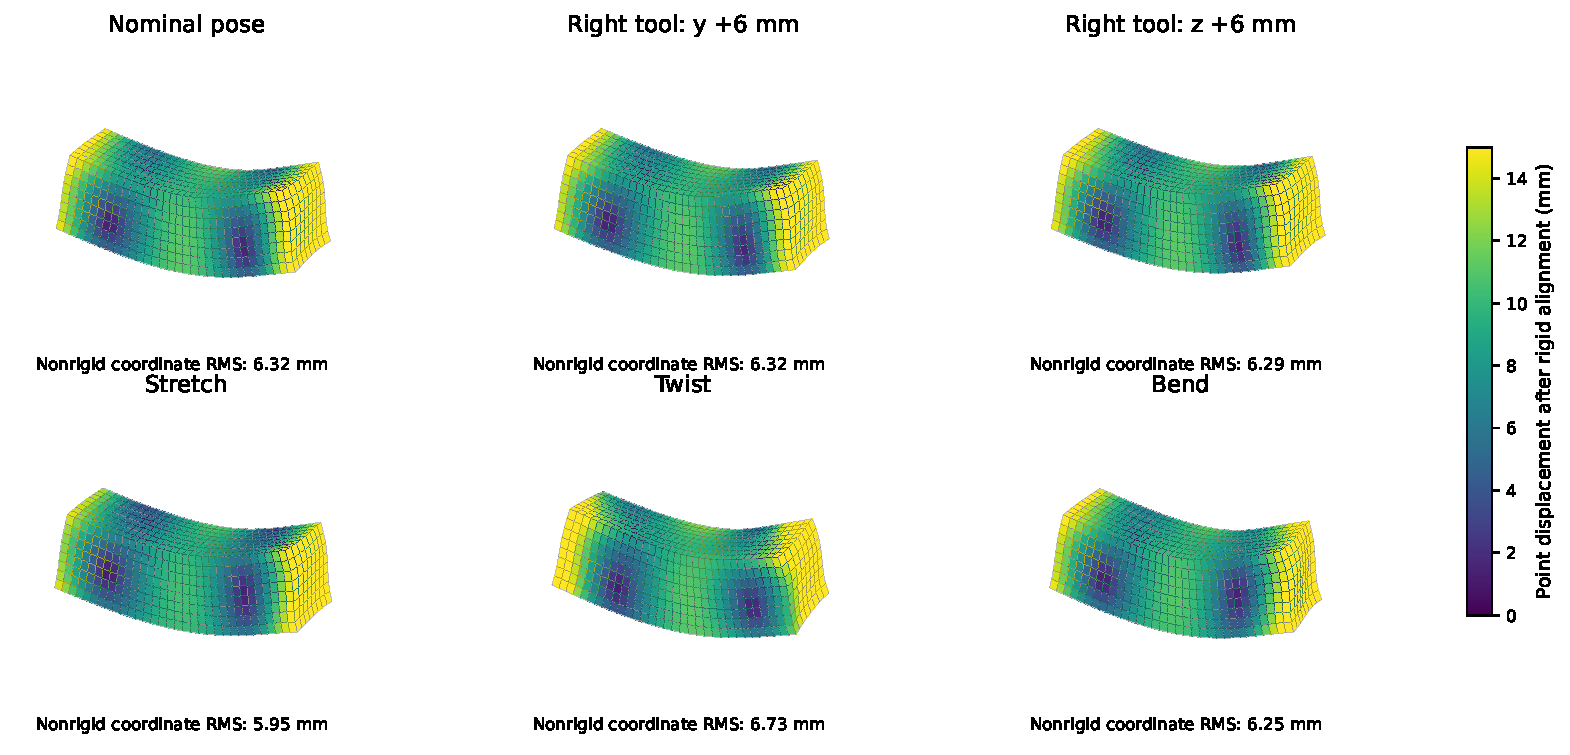
\includegraphics[width=\textwidth]{figures/scenarios.pdf}
\caption{Development reference geometry at actual deformation scale. The top row supplies the three observed configurations; the bottom row illustrates new positional interactions. Color measures displacement remaining after rigid alignment. The block has millimetre-scale nonrigid deformation, with no visual amplification.}
\label{fig:scenarios}
\end{figure*}


\section{Discussion}
The aim is reliable prediction under changed interactions, rather than recovering a unique physical label when observations do not identify it. A positional benchmark can expose explanatory ambiguities that remain hidden when models receive true force histories. Spatially factored models provide a direct mechanism for investigating these ambiguities, while strong learned and physical baselines establish when that structure is useful.

The present reference formulation describes settled equilibria. Interpolated equilibrium states are not dynamic ground truth, and impact, release, and dropping claims require separately validated trajectories. Results will be scoped to the material and environmental families actually evaluated.

\section*{LLM Usage Statement}
OpenAI Codex assisted with research planning, implementation, experiment execution and analysis, related-work lookup, figure preparation, and manuscript drafting. The manuscript and its experimental claims require review and approval by the human authors before submission.

{\small\bibliographystyle{ieeenat_fullname}\bibliography{references}}
\end{document}
